\documentclass[a4paper,12pt,Times]{article}
\usepackage{abakos}  %pacote com padrão da Abakos baseado no padrão da PUC
\usepackage{float}
%%%%%%%%%%%%%%%%%%%%%%%%%%%
%Capa da revista
%%%%%%%%%%%%%%%%%%%%%%%%%%

%\setcounter{page}{80} %iniciar contador de pagina de valor especificado
\newcommand{\monog}{Revista Abakós do Instituto de Ciências Exatas e de Informática Pontifícia Universidade Católica de Minas Gerais}
\newcommand{\monogES}{Model - Magazine Abakós - ICEI - PUC Minas}
\newcommand{\tipo}{Artigo }  % Especificar a seção tipo do trabalho: Artigo, Resumo, Tese, Dociê etc
\newcommand{\origem}{Brasil}
\newcommand{\editorial}{\textbf{Abakos}, Belo Horizonte,v. 1, n. 1, p. 00-00, Jul. 2013 - ISSN: 2316-9451}  % p. xx-xx – páginas inicial-final do artigo
% \newcommand{\lcc}{\scriptsize{Licença Creative Commons Attribution-NonCommercial-NoDerivs 3.0 Unported}}

%%%%%%%%%%%%%%%%%INFORMAÇÕES SOBRE AUTOR PRINCIPAL %%%%%%%%%%%%%%%%%%%%%%%%%%%%%%%
\newcommand{\AutorA}{Rafael Duarte Pereira}
\newcommand{\funcaoA}{}
\newcommand{\emailA}{rafael.pereira.1296852@sga.pucminas.br}
\newcommand{\cursA}{Graduação em Engenharia de Software da PUC Minas}
% 
% \newcommand{\AutorB}{Fernando José Rodrigues Cordeiro}
% \newcommand{\funcaoB}{Bacharel em Sistemas de Informação}
% \newcommand{\emailB}{fernandocordeiro@pucminas.br}
% \newcommand{\cursB}{Instituto de Ciências Exatas e de Informática da PUC Minas}
% 
% \newcommand{\AutorC}{Giovanni Candido da Silva}
% \newcommand{\funcaoC}{Bacharel em Sistemas de Informação}
% \newcommand{\emailC}{giovanni@pucminas.br}
% \newcommand{\cursC}{Instituto de Ciências Exatas e de Informática da PUC Minas}

% Definir macros para o nome da Instituição, da Faculdade, etc.
\newcommand{\univ}{Pontifícia Universidade Católica de Minas Gerais}

\newcommand{\keyword}[1]{\textsf{#1}}

\begin{document}
% %%%%%%%%%%%%%%%%%%%%%%%%%%%%%%%%%%
% %% Pagina de titulo
% %%%%%%%%%%%%%%%%%%%%%%%%%%%%%%%%%%

\begin{flushleft}

\begin{minipage} [c][5cm][b]{16.5cm} % a primeira minipágina tem uma altura de 1.5cm e uma largura de 2.3cm.
% comando que introduz o logo da escola que nesta altura já terá de estar na pasta imagens que 
%por sua vez está na pasta onde se guardou o arquivo tex. E introduzimos essa imagem com a mesma altura da minipage.

\includegraphics[scale=1.1]{figuras/pucmg.png} 
\end{minipage}

 \vspace{0cm} {
 \singlespacing \Large{\monog \symbolfootnote[1]{Artigo apresentado à Revista Abakos} \\ }
  \normalsize{\monogES}
 }
\end{flushleft}
\begin{flushright}
\singlespacing 
\normalsize{\AutorA \footnote{\funcaoA \cursA, \origem -- \emailA }} \\
% \normalsize{\AutorB \footnote{\funcaoB, E-mail:\emailB \\ \cursB, \origem. }} \\
% \normalsize{\AutorC \footnote{\funcaoC, E-mail:\emailC \\ \cursC, \origem. }} \\
% \normalsize{\AutorD \footnote{\funcaoD \\ Pais de origem: \origemD. E-mail: \emailD}} \\
%deixar com o valor `0` e usar o '*' no inicio da frase
% \symbolfootnote[0]{Artigo recebido em 10 de julho de 1983 e aprovado em 29 de maio 2012}
\end{flushright}
\thispagestyle{empty}
\begin{abstract}
\noindent
Algoritmos baseados em grafos são usados em diversas áreas para auxiliar nas resoluções de inúmeros problemas.
Um caminho simples em um grafo direcionado é um caminho onde não há repetição de vértices Em grafos
simples, pode-se representar um caminho apenas pela sequência de vértices (uma vez que só pode existir uma única aresta
entre cada par de vértices).
Encontrar caminhos disjuntos em um grafos simples é um problemas com mais de uma solução possível. 
O presente trabalho irá apresentar a implementação de uma solução que apresenta o máximo de caminhos disjuntos em um grafo direcionado simples.
\\\textbf{\keyword{Palavras-chave: }}Vetices. Caminhos. Grafo. Método. Implementação 
\end{abstract}

\selectlanguage{brazilian}
 \onehalfspace  % espaçamento 1.5 entre linhas
 \setlength{\parindent}{1.25cm}

%%%%%%%%%%%%%%%%%%%%%%%%%%%%%%%%%%%%%%%%%%%%%%%%%
%% INICIO DO TEXTO
%%%%%%%%%%%%%%%%%%%%%%%%%%%%%%%%%%%%%%%%%%%%%%%%%

%%%%%%%%%%%%%%%%%%%%%%%%%%%%%%%%%%%%%%%%%%%%%%%%%%%%%%%%%%%%%%%%%%%%%%%%%%%%%%%%%%%%%%%%%%%%%%%%%%%%%%%
%%%%%%%%%%%%%% Template de Artigo Adaptado para Trabalho de Diplomação do ICEI %%%%%%%%%%%%%%%%%%%%%%%%
%% codificação UTF-8 - Abntex - Latex -  							     %%
%% Autor:    Fábio Leandro Rodrigues Cordeiro  (fabioleandro@pucminas.br)                            %% 
%% Co-autor: Prof. João Paulo Domingos Silva  e Harison da Silva                                     %%
%% Revisores normas NBR (Padrão PUC Minas): Helenice Rego Cunha e Prof. Theldo Cruz                  %%
%% Versão: 1.0     13 de março 2014                                                                  %%
%%%%%%%%%%%%%%%%%%%%%%%%%%%%%%%%%%%%%%%%%%%%%%%%%%%%%%%%%%%%%%%%%%%%%%%%%%%%%%%%%%%%%%%%%%%%%%%%%%%%%%%

\section{\esp Implementação}

Para a implementação da solução foi utilizado uma adaptação do algoritmo de fluxo máximo Ford-Fulkerson \cite{site} onde foi definido o fluxo máximo como 1. Para cada rede de fluxo gerada faz-se uma busca em largura partindo do vértice s (vértice definido como origem do grafo) armazenamento em um vetor quais são os pais de cada vértice. Uma vez finalizada a busca precorre o vetor de pais partindo do vértice t (vértice definido como destino do grafo) adicionando o pai de cada vértice no começo de uma lista para definir qual foi o caminho percorrido pela busca. O método se repete até que a busca não consiga encontrar o vértice t e retorna um conjunto de de possíveis caminhos disjuntos de s para t.

O método foi implementado em Java utilizando o paradigma da orientação à objetos. Nesta implementação o grafo é um objeto que armazena em seu interior uma matriz de adjacência, o vértice de origem (s) e o vértice de destino (t), além do número total de vértices. A figura \ref{impl-grafo} mostra a implementação do código responsável por armazenar um grafo

\begin{figure}[H]
    \centering
    \caption{Implementação da classe grafo}
    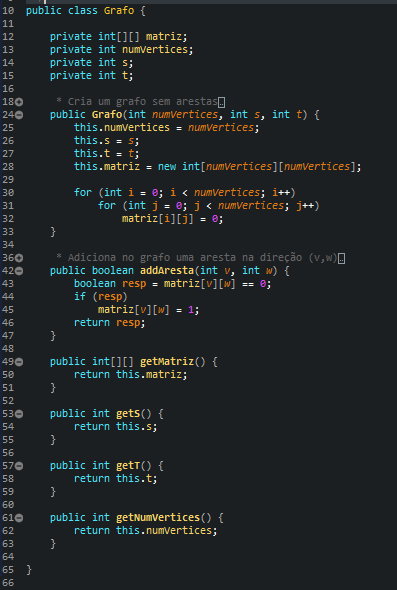
\includegraphics[width=0.6\textwidth]{figuras/grafoClass.png}
    \label{impl-grafo}
\end{figure}

A parte responsável por encontrar os caminhos conta com dois métodos, uma busca em largura que passa uma única vez em um vértice e que retorna um vetor indicando os pais de um vértice (Figura \ref{busca-largura}) e outro que a partir do vetor retornado pela busca monta os caminhos e gera uma nova rede de fluxo para realizar outra busca. O método só para quando a busca não encontra um caminho para t e retorna os caminhos encontrados (Figura \ref{encontrar-caminhos}).

\begin{figure}[H]
    \centering
    \caption{Implementação da busca em largura}
    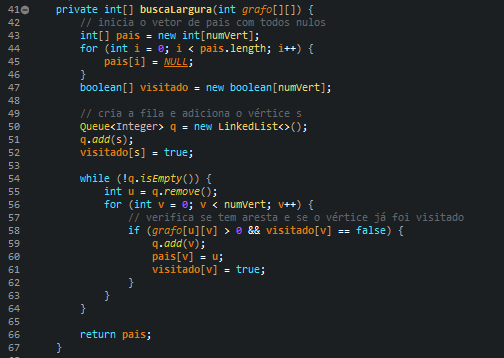
\includegraphics[width=0.7\textwidth]{figuras/buscaLargura.png}
    \label{busca-largura}
\end{figure}

\begin{figure}[H]
    \centering
    \caption{Implementação do método de encontrar caminhos}
    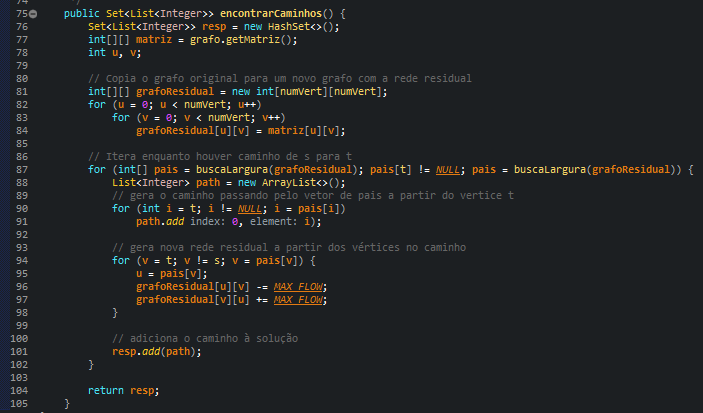
\includegraphics[width=0.7\textwidth]{figuras/encontrarCaminhos.png}
    \label{encontrar-caminhos}
\end{figure}

\section{\esp Testes e resultados}

Para os testes foram utilizados três grafos direcionados simples, isto é sem ciclos e sem arestas paralelas. Os grafos estavam salvos em aquivos de texto com  a seguinte estrutura:
na primeira linha o numero de vértices, o vértice de origem e o vértice de destino na respectiva ordem separados por espaços e nas linhas subsequentes  estava as arestas, uma em cada linha, com vértice de origem e vértice de destino nessa respectiva ordem separadas por espaços.

Os grafos testados foram os seguintes

\subsection{\esp Grafo 1}

O grafo G1 apresenta seis vértices e 11 arestas e os caminhos a serem procurados pelo algoritmo partiam do vértice 0 ao vértice 5 conforme a Figura \ref{grafo1}.
\begin{figure}[H]
	\centering	
	\caption[\hspace{0.1cm}]{G1}
	\vspace{-0.4cm}
	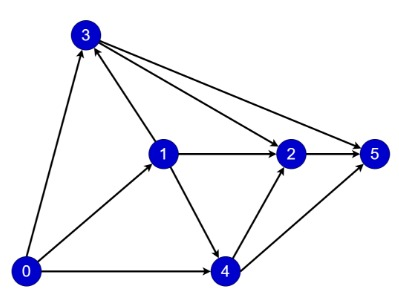
\includegraphics[width=0.6\textwidth]{figuras/grafo1.png}
	\label{grafo1}
\end{figure}
    
Para tal grafo existem no máximo três caminhos disjuntos conforme está marcado na Figura \ref{caminhos-grafo1} e, o método foi capaz de encontrar os três caminhos conforme indicado na Figura \ref{solucao-grafo1} extraída do console da IDE

\begin{figure}[H]
    \centering
    \caption{Caminhos disjuntos de G1}
    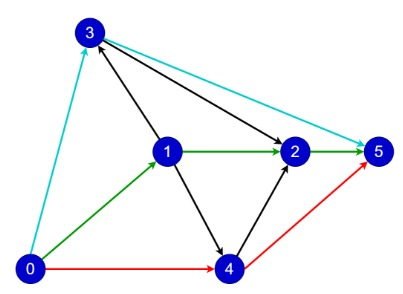
\includegraphics[width=0.6\textwidth]{figuras/caminhos-grafo1.png}
    \label{caminhos-grafo1}
\end{figure}


\begin{figure}[H]
    \centering
    \caption{Resultados de G1}
    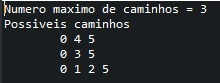
\includegraphics[width=0.6\textwidth]{figuras/solucao-grafo1.png}
    \label{solucao-grafo1}
\end{figure}
    
\subsection{\esp Grafo 2}

O grafo G2 apresenta nove vértices e 13 arestas e os caminhos a serem procurados pelo algoritmo partiam do vértice 0 ao vértice 8 conforme a Figura \ref{grafo2}

\begin{figure}[H]
    \centering
    \caption{G2}
    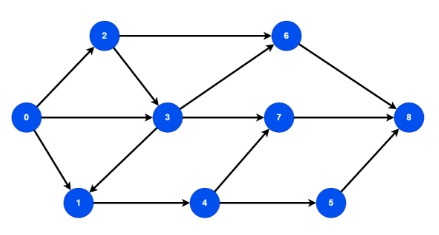
\includegraphics[width=0.6\textwidth]{figuras/grafo2.png}
    \label{grafo2}
\end{figure}

Para tal grafo existem no máximo três caminhos disjuntos conforme está marcado na Figura \ref{caminhos-grafo2} e, o método foi capaz de encontrar os três caminhos conforme indicado na Figura \ref{solucao-grafo2} extraída do console da IDE

\begin{figure}[H]
    \centering
    \caption{Caminhos disjuntos de G2}
    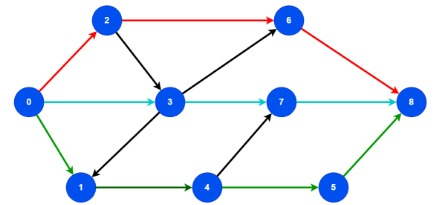
\includegraphics[width=0.6\textwidth]{figuras/caminhos-grafo2.png}
    \label{caminhos-grafo2}
\end{figure}


\begin{figure}[H]
    \centering
    \caption{Resultados de G2}
    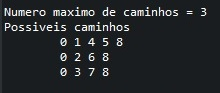
\includegraphics[width=0.6\textwidth]{figuras/solucao-grafo2.png}
    \label{solucao-grafo2}
\end{figure}
    
\subsection{\esp Grafo 3}

O grafo G3 apresenta 12 vértices e 21 arestas e os caminhos a serem procurados pelo algoritmo partiam do vértice 0 ao vértice 11 conforme a Figura \ref{grafo3}

\begin{figure}[H]
    \centering
    \caption{G3}
    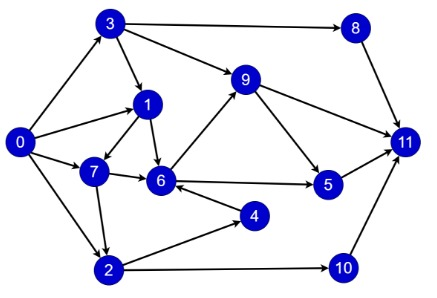
\includegraphics[width=0.6\textwidth]{figuras/grafo3.png}
    \label{grafo3}
\end{figure}

Para tal grafo existem no máximo três caminhos disjuntos conforme está marcado na Figura \ref{caminhos-grafo3} e, o método foi capaz de encontrar os três caminhos conforme indicado na Figura \ref{solucao-grafo3} extraída do console da IDE

\begin{figure}[H]
    \centering
    \caption{Caminhos disjuntos de G3}
    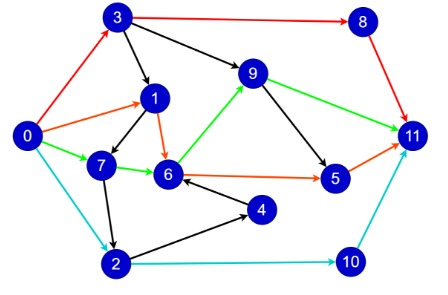
\includegraphics[width=0.6\textwidth]{figuras/caminhos-grafo3.png}
    \label{caminhos-grafo3}
\end{figure}


\begin{figure}[H]
    \centering
    \caption{Resultados de G3}
    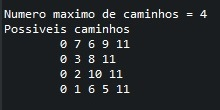
\includegraphics[width=0.6\textwidth]{figuras/solucao-grafo3.png}
    \label{solucao-grafo3}
\end{figure}



\section{\esp Conclusão}

Pode-se concluir que a solução implementada é capaz de achar possíveis caminhos disjuntos em grafos simples com um custo no pior caso de O(n), ou seja, o algoritmo é linear ao número de vértices de um grafo.

%%%%%%%%%%%%%%%%%%%%%%%%%%%%%%%%%%%
%% FIM DO TEXTO
%%%%%%%%%%%%%%%%%%%%%%%%%%%%%%%%%%%

% \selectlanguage{brazil}
%%%%%%%%%%%%%%%%%%%%%%%%%%%%%%%%%%%
%% Inicio bibliografia
%%%%%%%%%%%%%%%%%%%%%%%%%%%%%%%%%%%

 \newpage
 \singlespace{
 \bibliographystyle{abntex2-alf}
 \bibliography{bibliografia}
 }

\end{document}